\documentclass[a4paper, 14pt,russian]{extarticle}

\usepackage[russian]{babel}
\usepackage[T2A]{fontenc}
\usepackage[utf8]{inputenc}
%Соответствующий математический шрифт для Times new roman
\usepackage{newtxmath}
\usepackage{fontspec} 
\usepackage{multirow}
%\usepackage{polyglossia}
%Times new roman
\defaultfontfeatures{Ligatures={TeX},Renderer=Basic} 
\setmainfont[Ligatures={TeX,Historic}]{Times New Roman}
\setmainfont{Times New Roman}
\setsansfont{Arial}
\setmonofont{Courier New}
\newfontfamily\cyrillicfont[Script=Cyrillic]{Times New Roman}
\newfontfamily\cyrillicfontsf[Script=Cyrillic]{Arial}
\newfontfamily\cyrillicfonttt[Script=Cyrillic]{Courier New}

%\setdefaultlanguage{russian}

%Геометрия
\usepackage{geometry}
\geometry{top=20mm}
\geometry{bottom=15mm}
\geometry{left=20mm}
\geometry{right=15mm}
\usepackage{setspace}
%Нормальные дроби через запятую
\usepackage{ncccomma}

\newcommand{\changefont}{%
	\fontsize{12}{11}\selectfont
}

%Заголовки
\usepackage{fancyhdr}
\pagestyle{fancy}
\fancyhf{}
%\renewcommand{\sectionmark}[1]{\markright{#1}}
\fancyhead[R]{\changefont \slshape \leftmark}
\fancyhead[L]{\changefont \slshape \rightmark}
%\newcommand{\ssubsection}[1]{\subsection*{#1}
%	\addcontentsline{toc}{subsection}{#1}
%	\markright{#1}{}}
\cfoot{\thepage}

%\полуторный интервал
\setstretch{1.15}
\setlength{\parindent}{1.25cm}

\usepackage{amsmath, amsfonts, mathtools}
\usepackage{physics}
\usepackage{indentfirst}
\usepackage{xcolor}
\usepackage{alltt}
\usepackage{graphicx}
\usepackage{wrapfig}
\usepackage{pgfplots}

%Настройка ссылок
\usepackage{hyperref}
%\usepackage{upgreek}
%\renewcommand{\beta}{\upbeta}
\hypersetup{
	colorlinks,
	citecolor=black,
	filecolor=black,
	linkcolor=black,
	urlcolor=black
}
\usepackage{caption}
\DeclareCaptionLabelSeparator{dot}{. }
\captionsetup{justification=centering,labelsep=dot}
\usepackage{titlesec}

%Формат заголовков
\titleformat{\section}{\bfseries\filcenter\Large}{\thesection}{1em}{}
\titleformat{\subsection}{\bfseries\filcenter\large}{\thesubsection}{1em}{}
\titleformat{\subsubsection}{\bfseries\filcenter\normalsize}{\thesubsubsection}{1em}{}

\usepackage{chngcntr}

%Включить в нумерацию картинок раздел
\counterwithin{figure}{section}

%Листинги кода и их стили
\usepackage{listings}
\usepackage{minted}
\lstdefinestyle{c++} {
	language=C++,
	breaklines=true,
	frame=single,
	numbers=left,
	basicstyle=\footnotesize\ttfamily,
	keywordstyle=\bfseries\color{green!40!black},
	commentstyle=\itshape\color{purple!40!black},
	identifierstyle=\color{blue},
	backgroundcolor=\color{gray!10!white},
}

\lstdefinestyle{python}{
	language=Python,
	breaklines=true,
	frame=single,
	numbers=left,
	keywordstyle=\bfseries\color{green!40!black},
	frame=lines,
	basicstyle=\footnotesize\rmfamily
}

\lstdefinestyle{cmd}{
	breaklines=true,
	frame=single,
	basicstyle=\footnotesize\ttfamily,
	frame=lines
	basicstyle=\footnotesize
}
\usepackage{tikz}
\usepackage{tkz-base}
\usetikzlibrary{quotes,angles}
\usetikzlibrary {arrows.meta}
%\usepackage{tkz-euclide}
\usetikzlibrary{calc}
\usetikzlibrary{shapes.geometric, shapes.misc, arrows}

\tikzstyle{startstop} = [rectangle, rounded corners, 
minimum width=3cm, 
minimum height=1cm,
text centered, 
draw=black]

\tikzstyle{io} = [trapezium, 
trapezium stretches=true, % A later addition
trapezium left angle=70, 
trapezium right angle=110, 
minimum width=3cm, 
minimum height=1cm, text centered, 
draw=black]

\tikzstyle{process} = [rectangle, 
minimum width=3cm, 
minimum height=1cm, 
text centered, 
text width=5cm, 
draw=black]

\tikzstyle{decision} = [diamond, 
minimum width=3cm, 
minimum height=1cm, 
text centered, 
draw=black]
\tikzstyle{arrow} = [thick,->,>=stealth]

\tikzstyle{startfor} = [chamfered rectangle, 
chamfered rectangle corners={north west, north east},
minimum width=3cm, 
minimum height=1cm, 
text centered, 
draw=black]

\tikzstyle{endfor} = [chamfered rectangle, 
chamfered rectangle corners={south west, south east},
minimum width=3cm, 
minimum height=1cm, 
text centered, 
draw=black]
\tikzstyle{arrow} = [thick,->,>=stealth]

\begin{document}
	
	\begin{titlepage}
	\newpage
	\begin{center}
		
\includegraphics[width=\textwidth]{png/tit.png}
		Институт информационных и вычислительных технологий \\
		Кафедра управления и интеллектуальных технологий
		\vspace{1.25cm}
	\end{center}
	
	\vspace{1.2em}
	
	\begin{center}
		%\textsc{\textbf{}}
		\begin{spacing}{1}
			{\Large Лабораторная работа №2\linebreak
				По дисциплине <<Теория автоматического управления>> \\}
			\large{\bf<<Анализ динамики нелинейных систем методом фазовой плоскости>>}
		\end{spacing}
	\end{center}
	
	\vspace{5em}
	
	
	\vspace{6em}
	
	\noindent Выполнили студенты: Михайловский М., Томчук В. \\
	Группа: А-03-21 \\
	Бригада: 1\\
	Проверил: Деменьтьев В.\,Ю.
	
	
	\vspace{\fill}
	
	\begin{center}
		Москва 2024
	\end{center}
	
\end{titlepage}
	\pagenumbering{arabic}
	\setcounter{page}{2}
	\tableofcontents
	\newpage
	

	\section{Нахождение дискретной передаточной функции}
	
	Рассматривается импульсная схема автоматического управления (ИСАУ), со следующей структурной схемой (рис. \ref{ss}).
	
	Для заданной формы импульса на выходе формирователя импульсов необходимо найти дискретную передаточную функцию формирователя. На вход этого элемента подаётся последовательность дельта-функций: 
	\begin{equation*}
		x^{*}(t) = x(t) \sum_{l=0}^\infty \delta(t-lT).	
	\end{equation*}
	
	Переходной процесс при подаче дельта-функции (то есть весовая характеристика этого звена) имеет вид представленный на рис. \ref{w}.
	
	
	\begin{center}
		\begin{tikzpicture}
			% Sum shape
			\node[draw,
			circle,
			minimum size=1cm
			] (sum) at (0,0){};
			\draw (sum.north east) -- (sum.south west)
			(sum.north west) -- (sum.south east);
			%\draw[fill=black] (sum.center) -- (sum.south west) arc (sum.south east) -- (sum.center);
			\draw[fill=black] (0,0) -- (-135:0.5cm) arc (-135:-45:0.5cm) -- cycle;
			
			\draw [-{Latex[length=3mm]}, thick] ($ (sum) + (-2cm,0) $) -- (sum) node[midway, above] {$g(t)$};
			
			\node (IIE)[draw, 
			minimum width = 1.6cm,
			minimum height = 1.2cm,
			right=2cm] at (sum) {};   
			\draw [thick] ($(IIE.west) + (0.3cm,-0.4cm)$) -- ($(IIE.east) + (-0.3cm, -0.4cm)$);
			\draw [-{Latex[length=3mm]}, thick] ($ (IIE.center) + (0, -0.4cm) $) -- ($ (IIE.north) + (0, -0.1cm) $);
			
			\node (form) [draw, 
			minimum width = 1.6cm,
			minimum height = 1.2cm,
			right=2.5cm] at (IIE) {$W_\text{ф}(p)$};   
			
			\node (nepr) [draw, 
			minimum width = 1.6cm,
			minimum height = 1.2cm,
			right=2.5cm] at (form) {$W_\text{н}(p)$};   
			
			\draw [-{Latex[length=3mm]}, thick] (sum) -- (IIE) node [midway,above]{$x(t)$};
			\draw [-{Latex[length=3mm]}, thick] (IIE) -- (form) node [midway,above]{$x^{*}(t)$};
			\draw [-{Latex[length=3mm]}, thick] (form) -- (nepr) node [midway,above]{$x^{*}_\text{ф}(t)$};
			\draw[-{Latex[length=3mm]}, thick] (nepr.east) -- ++ (1.25cm,0) 
			node[midway](output){}node[midway,above]{$y(t)$};
			\draw[-{Latex[length=3mm]}, thick]  (output.center) |- ($ (form) + (0, -1.5cm) $) -| (sum.south);
		\end{tikzpicture}
		\captionof{figure}{Структурная схема импульсной системы автоматического управления}
		\label{ss}
	\end{center}
	
	\begin{center}
		\begin{tikzpicture}
			\tkzInit[xmax=4,ymax=4,xmin=0,ymin=0];
			\tkzDrawX[label=$t$];
			\tkzLabelX[orig=true];
			\tkzDrawY[label=$x^{*}_\text{ф}$];
			\tkzLabelY[orig=true];
			\draw [thick] (0,0) -- (1,2);
			\draw [thick] (1, 2) -- (2, 3);
			\draw [thick] (2, 3) -- (2, 1);
			\draw [thick] (2, 1) -- (3, 0);
			\draw [thick] (3, 0) -- (4, 0);
			\draw [dashed] (0, 1) -- (2, 1);
			\draw [dashed] (0, 2) -- (1, 2);
			\draw [dashed] (0, 3) -- (2, 3);
			\draw [dashed] (1, 0) -- (1, 2);
			\draw [dashed] (2, 0) -- (2, 1);
			
		\end{tikzpicture}	
		\captionof{figure}{Весовая характеристика формирователя импульсов}
		\label{w}
	\end{center}
	
	
	Этот сигнал можно представить в следующем виде (\ref{w(t)}):
	\begin{multline}
		w_\text{ф}(t) = 2t\cdot 1_0 (t) - (t-1)\cdot 1_0 (t-1) - (2t-2)\cdot 1_0 (t-2) + (t-3)\cdot 1_0 (t-3) = \\ = 2t\cdot 1_0 (t) - (t-1)\cdot 1_0 (t-1) - [2(t-2)+2]\cdot 1_0 (t-2) + (t-3)\cdot 1_0 (t-3)
		\label{w(t)}
	\end{multline}
	
	Тогда передаточная функция формирователя примет следующий вид:
	\begin{equation}
		W_\text{ф}(p) = \mathcal{L}[w_\text{ф}(t)] = \frac{2}{p^2} - \frac{1}{p} e^{-pT} - \left(\frac{2}{p^2} + \frac{2}{p}\right)e^{-2pT} + \frac{1}{p^2}e^{-3pT}
		\label{Wf}
	\end{equation}
	
	Именно такой результат был получен в ходе лабораторной работы и проверен в программе, рис. \ref{Wf_screenshot}.
	
	\begin{figure}
		\centering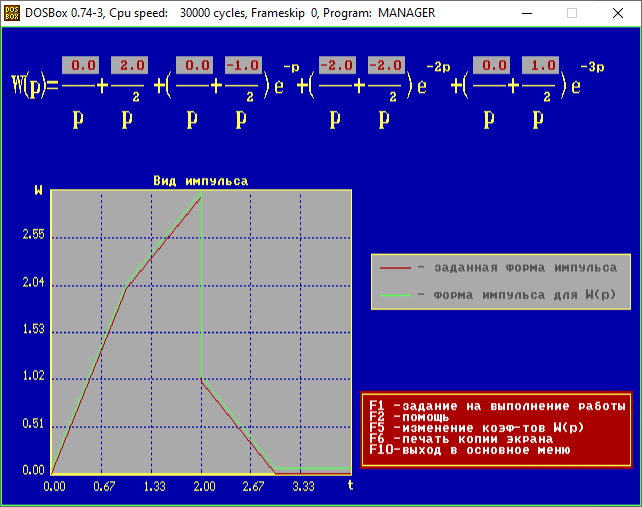
\includegraphics[width=.6\textwidth]{png/wf.png}
		\caption{Проверка полученной передаточной функции формирователя в программе}
		\label{Wf_screenshot}
	\end{figure}
	
	\section{Влияние квантования $T$ на свойства ИСАУ}
	
	Мы будем исследовать поведение ИСАУ со следующей непрерывной частью:
	\begin{equation}
		W_\text{нч}(p) = \frac{ 0,2 (1+2p)}{ p (1+p) (1+3p)^2 } = \frac{ 0,4p + 0,2 } { 9p^4 + 15p^3 + 7p^2 + p }
		\label{Wnch}
	\end{equation}
	
	Передаточная функция формирователя имеет вид (\ref{Wf2}). Таким образом, последовательность дельта-функций, поступающих с идеального импульсного элемента, модулируются в последовательность прямоугольных импульсов с длительностью равной периоду квантования $T$.
	\begin{equation}
		W_\text{ф}(p) = \frac{1-e^{-pT}}{p}
		\label{Wf2}
	\end{equation}
	
	\subsection{Динамические свойства}
	
	Для исследования влияния периода квантования на показатели качества была собрана следующая схема для моделирования в среде Simintech: рис. \ref{scheme1}
	
	Период квантования изменялся в пределах от $T=0.01$ с до $T=0.5$ с. На рис. \ref{graph1}, \ref{graph2} представлены переходные процессы для этих значений периода квантования. Для меньшего периода визуальных различий в процессах не видно, но для $T=0.5$ отличие от процесса в непрерывной системе заметно.
	
	\begin{figure}
		\centering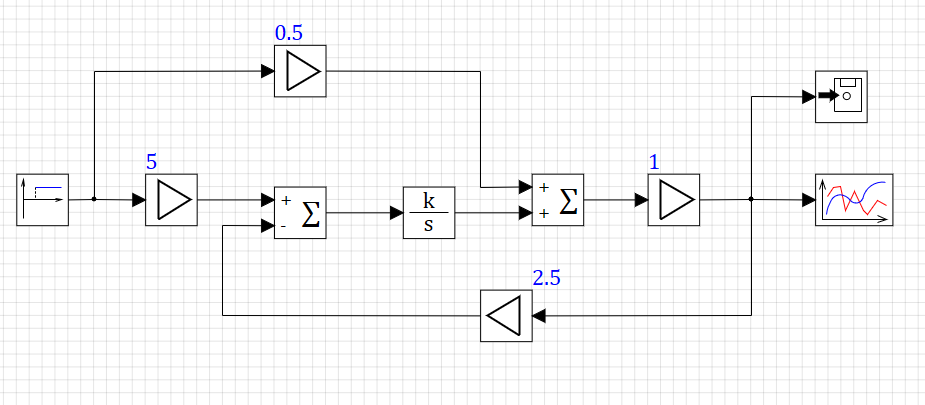
\includegraphics[width=.7\textwidth]{png/scheme1.png}
		\caption{Схема для исследования влияния квантования на показатели качества ИСАУ}
		\label{scheme1}
	\end{figure}
	
	\begin{figure}[h]
		\centering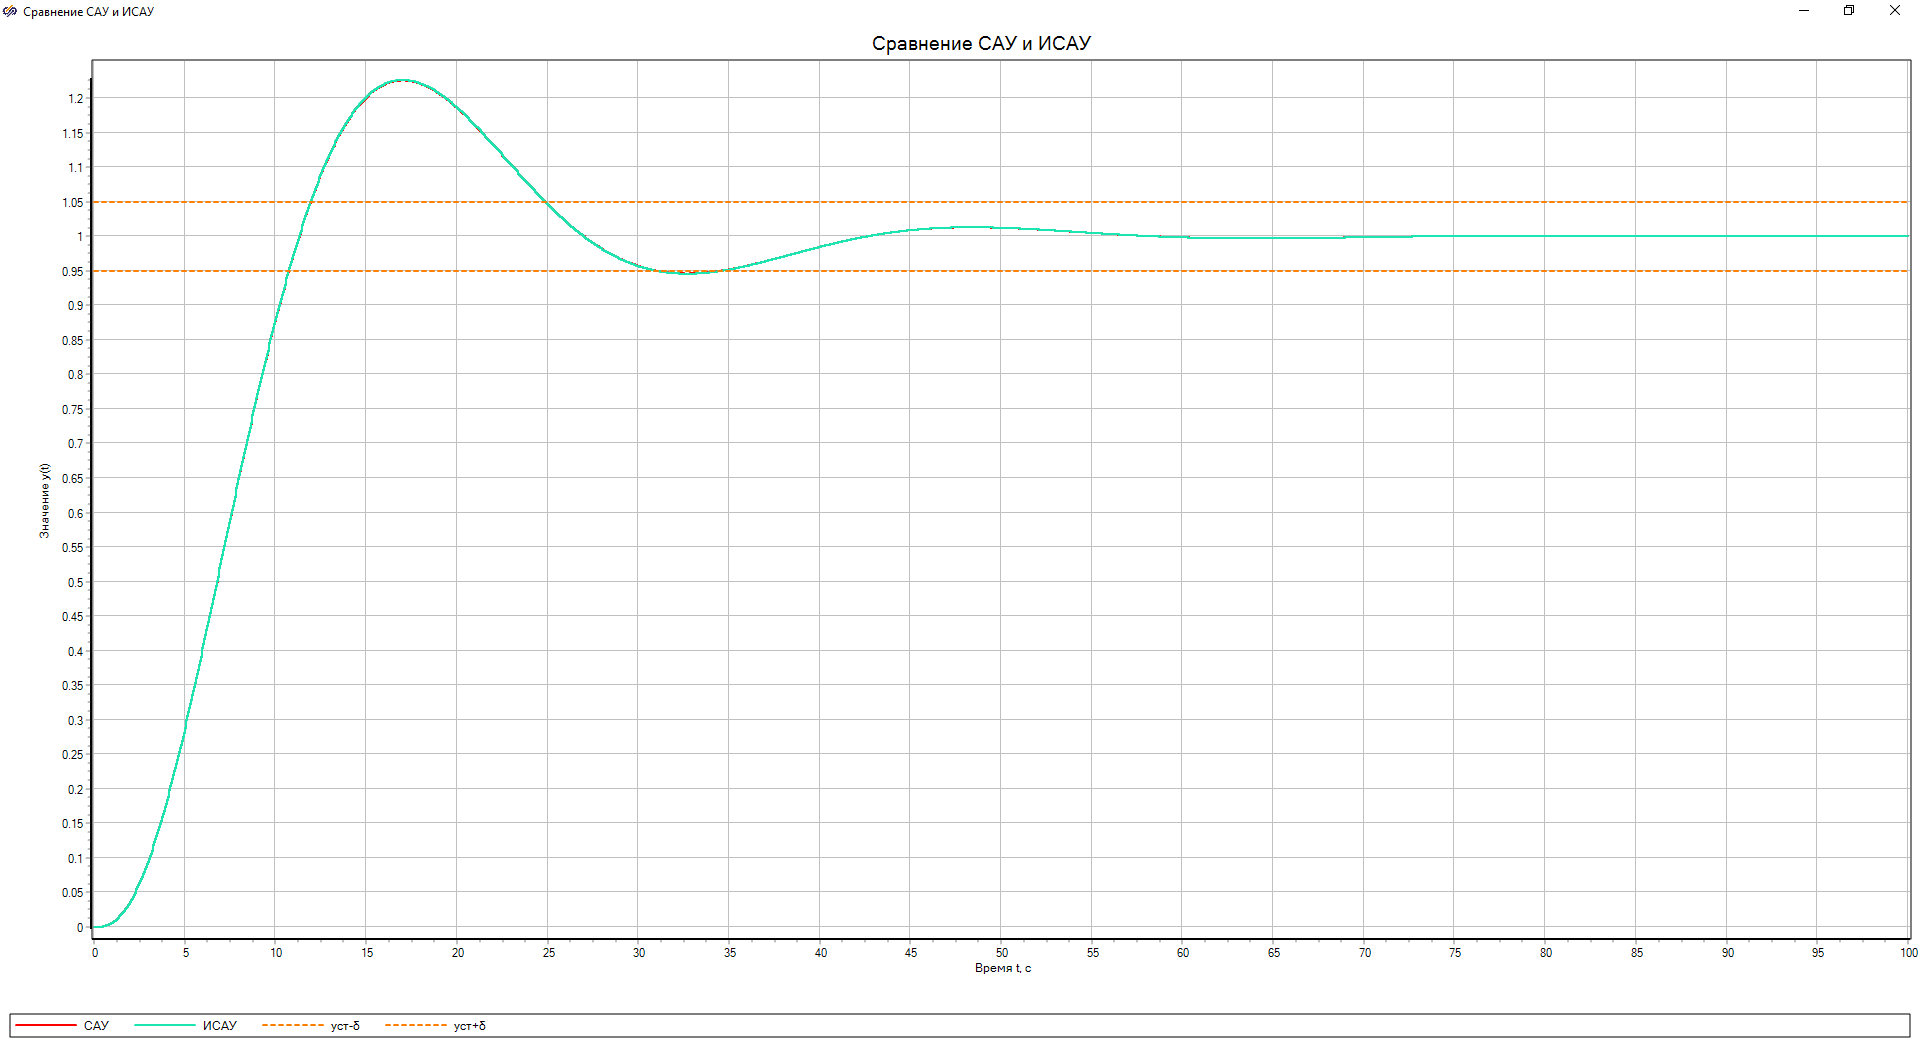
\includegraphics[width=.75\textwidth]{png/graph1.png}
		\caption{Переходной процесс САУ и ИСАУ при $T=0.01$ с}
		\label{graph1}
	\end{figure}
	
	\begin{figure}[h]
		\centering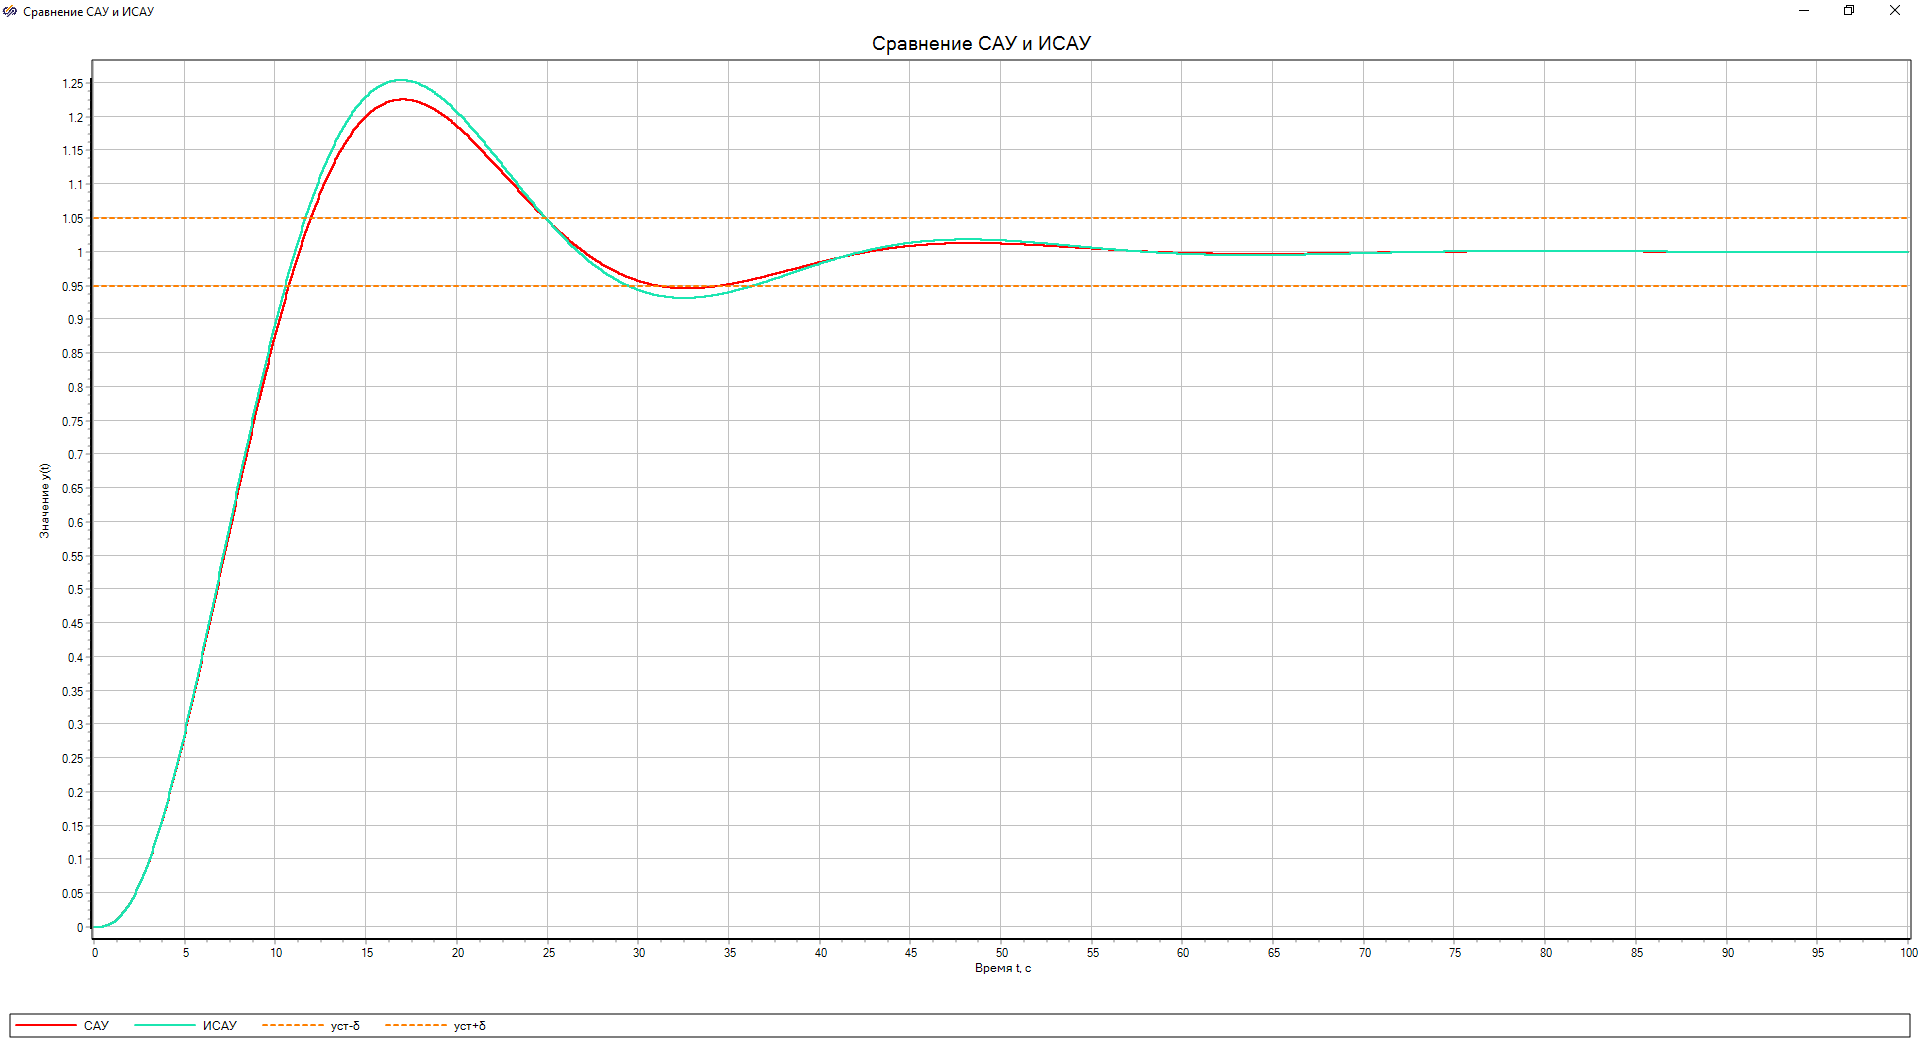
\includegraphics[width=.75\textwidth]{png/graph2.png}
		\caption{Переходной процесс САУ и ИСАУ при $T=0.5$ с}
		\label{graph2}
	\end{figure}
	

	
	\begin{table}
		\begin{tabular}{|c|cc|cc|}
			\hline
			Время квантования $T$, с & \multicolumn{2}{c|}{Время регулирования $\tau$, с} & \multicolumn{2}{c|}{Перерегулирование $\sigma$, \%} \\ \hline
			-                     & \multicolumn{1}{c|}{ИСАУ}   & Отличие от САУ & \multicolumn{1}{c|}{ИСАУ}  & Отличие от САУ \\ \hline
			0.01                  & \multicolumn{1}{c|}{34.65}  & 0.05           & \multicolumn{1}{c|}{18.43} & 0              \\ \hline
			0.05                  & \multicolumn{1}{c|}{34.85}  & 0.25           & \multicolumn{1}{c|}{18.57} & 0.14           \\ \hline
			0.1                   & \multicolumn{1}{c|}{35.06}  & 0.46           & \multicolumn{1}{c|}{18.77} & 0.34           \\ \hline
			0.25                  & \multicolumn{1}{c|}{35.65}  & 1.05           & \multicolumn{1}{c|}{19.35} & 0.92           \\ \hline
			0.5                   & \multicolumn{1}{c|}{36.38}  & 1.78           & \multicolumn{1}{c|}{20.26} & 1.83           \\ \hline
		\end{tabular}
		\caption{Влияние периода квантования на время регулирования и перерегулирование}
		\label{din_table}
	\end{table}
	
	Итоговые значения времени регулирования и перерегулирования, которые были получены в результате моделирования, приведены в табл. \ref{din_table}. 
	
	Как видно, чем выше период квантования $T$, тем менее хорошие динамические свойства имеет импульсная система, а именно процесс имеет более колебательный характер и дольше приходит к установившемуся режиму.
	
	Для малых периодов квантования процессы в САУ и ИСАУ протекают практически одинаково, и в предельном случае при $T\to 0$ эти процессы будут совпадать.
	
	\subsection{Ошибка регулирования}
	
	Как мы видели по характеру переходных процессов -- процессы в ИСАУ имели очень схожий характер с аналогичной непрерывной системой. Поэтому можно предположить, что ошибка регулирования в такой системе будет той же, что и в САУ.
	
	Для САУ как известно статическая ошибка будет равна нулю, поскольку система содержит интегратор, то есть является астатической.
	
	Кинетическая ошибка для САУ имеет следующий вид, где $k$ -- добротность системы.:
	\begin{multline}
		\Delta_\text{кин} = \left.\lim_{t\to \infty} \delta (t)\right| _{g(t) = t\cdot 1_0 (t)} = \lim_{p\to 0} p W_\delta (p) \cdot \frac{1}{p^2} = \\ = \lim_{p\to 0} \frac{1}{p}\cdot \frac{1}{1+\frac{B(p)}{pA(p)}} = \lim_{p\to 0} \frac{A(p)}{pA(p)+B(p)} = \frac{1}{k}
	\end{multline}
	
	В исследуемой системе имеем $\Delta_\text{кин} = \frac{1}{0,2} = 5$. Проверим это с помощью моделирования для системы с периодом квантования $T=0,5$ с. Схема для моделирования приведена на рис. \ref{scheme2}. Переходной процесс ошибки регулирования приведен на рис. \ref{graph3}.
	
	\begin{figure}
		\centering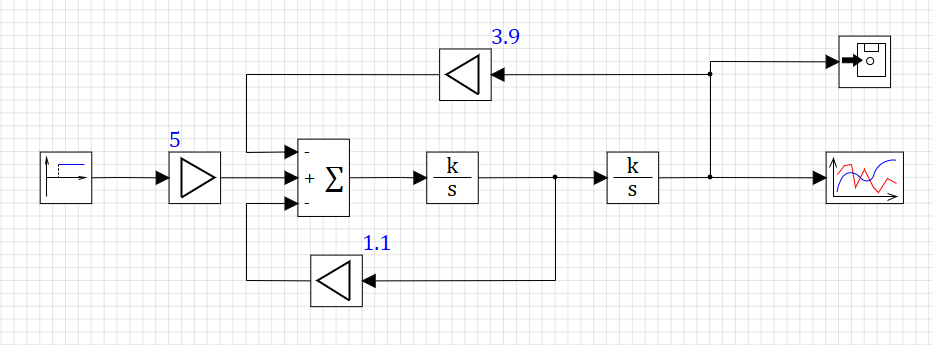
\includegraphics[width=.7\textwidth]{png/scheme2.png}
		\caption{Схема для моделирования ошибки регулирования}
		\label{scheme2}
	\end{figure}
	
	\begin{figure}
		\centering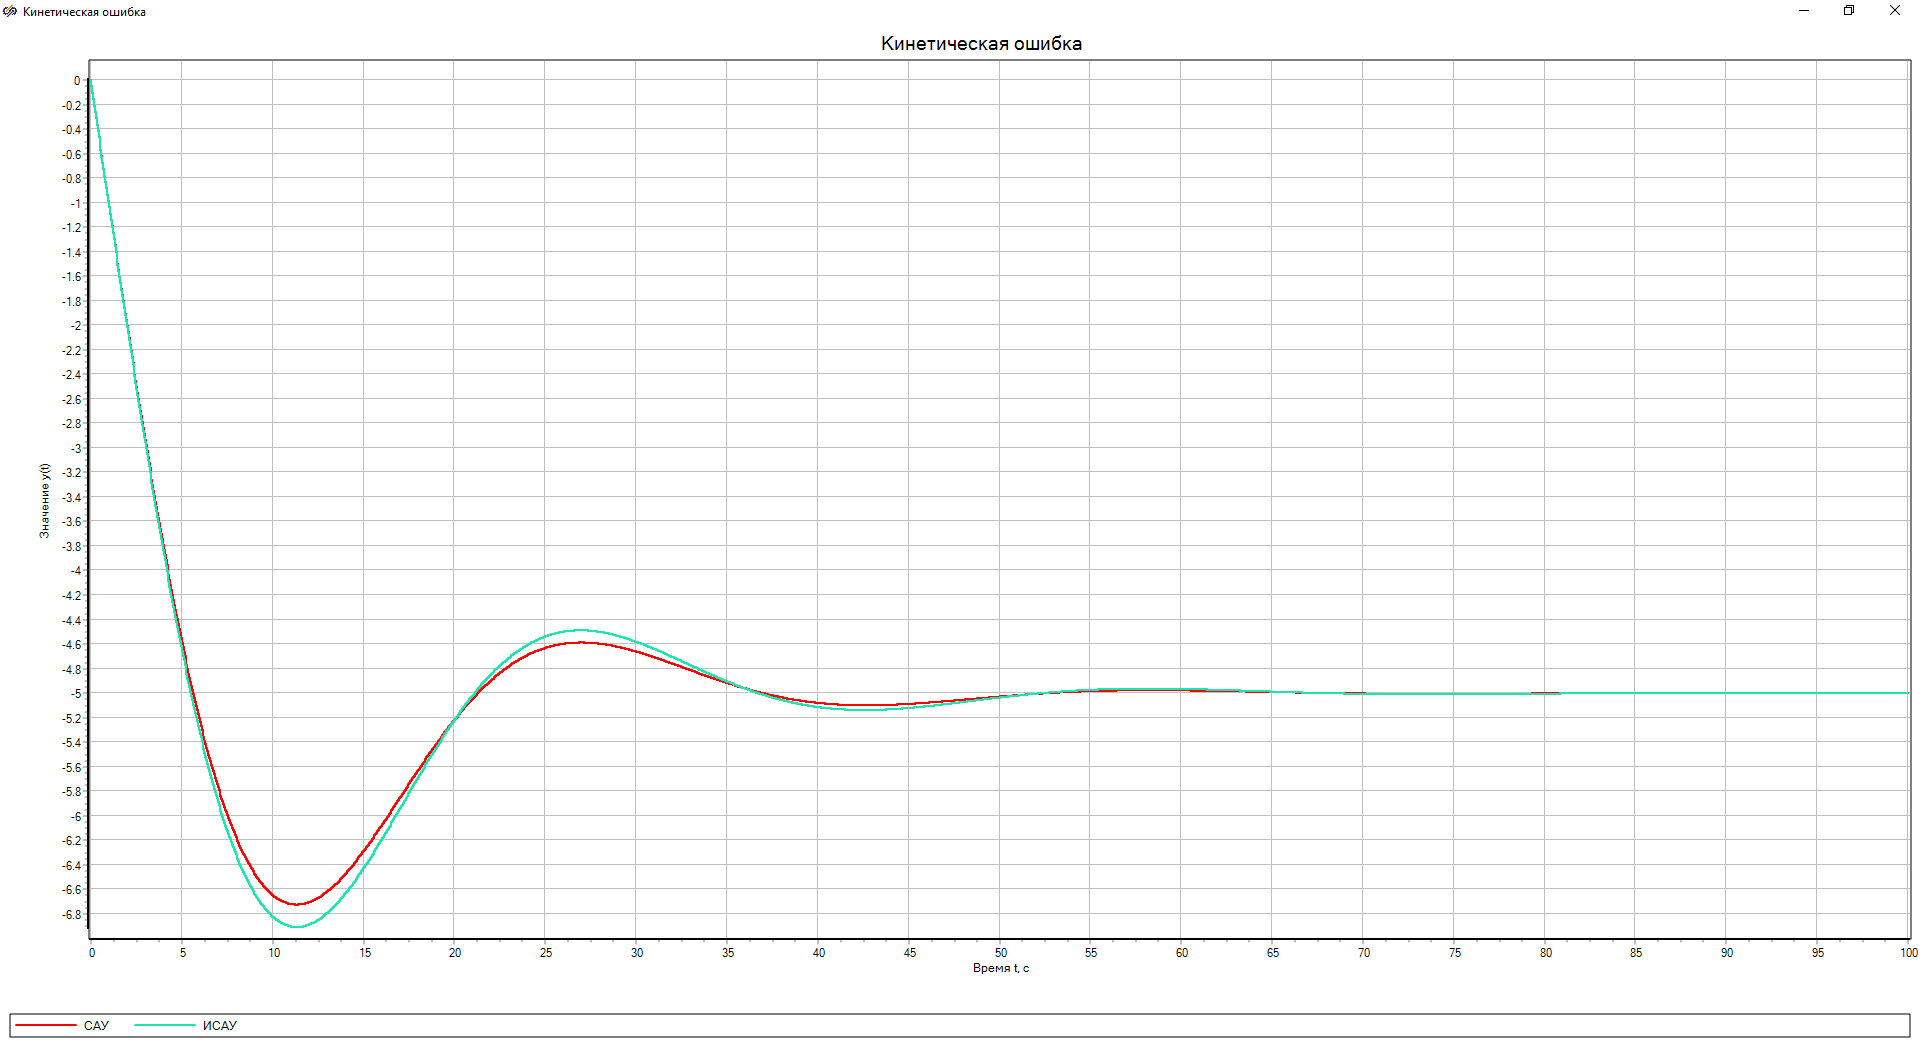
\includegraphics[width=.85\textwidth]{png/graph3.png}
		\caption{Переходной процесс ошибки регулирования для САУ и ИСАУ с $T=0,5$ с}
		\label{graph3}
	\end{figure}
	
	Как видим, установившееся значение ошибки совпадает для непрерывной и импульсной систем, и равняется 5. 
	
	Можем сделать вывод, что если устойчивость импульсной системы при данном периоде квантования сохраняется, то ошибка регулирования будет иметь то же значение, что и в соответствующей непрерывной системе.
	
	\subsection{Область устойчивости}
	
	Исследуем влияние на границу устойчивости системы по добротности $k$ для разных значений постоянной времени $T_1$, которая стоит в числителе передаточной функции непрерывной части и периода квантования $T$.
	
	Для этого соберём схему, приведенную на рис. \ref{scheme3} и будем искать значение $k=k_\text{пр}$ при котором наблюдаются незатухающие колебания следующего вида: рис. \ref{graph4}.
	
	\begin{figure}
		\centering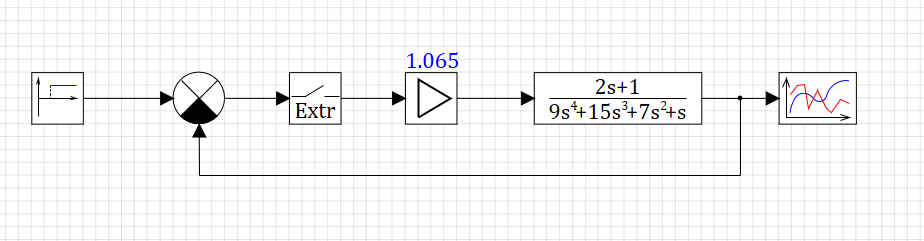
\includegraphics[width=.7\textwidth]{png/scheme3.png}
		\caption{Схема для поиска границы устойчивости}
		\label{scheme3}
	\end{figure}
	
	\begin{figure}[!h]
		\centering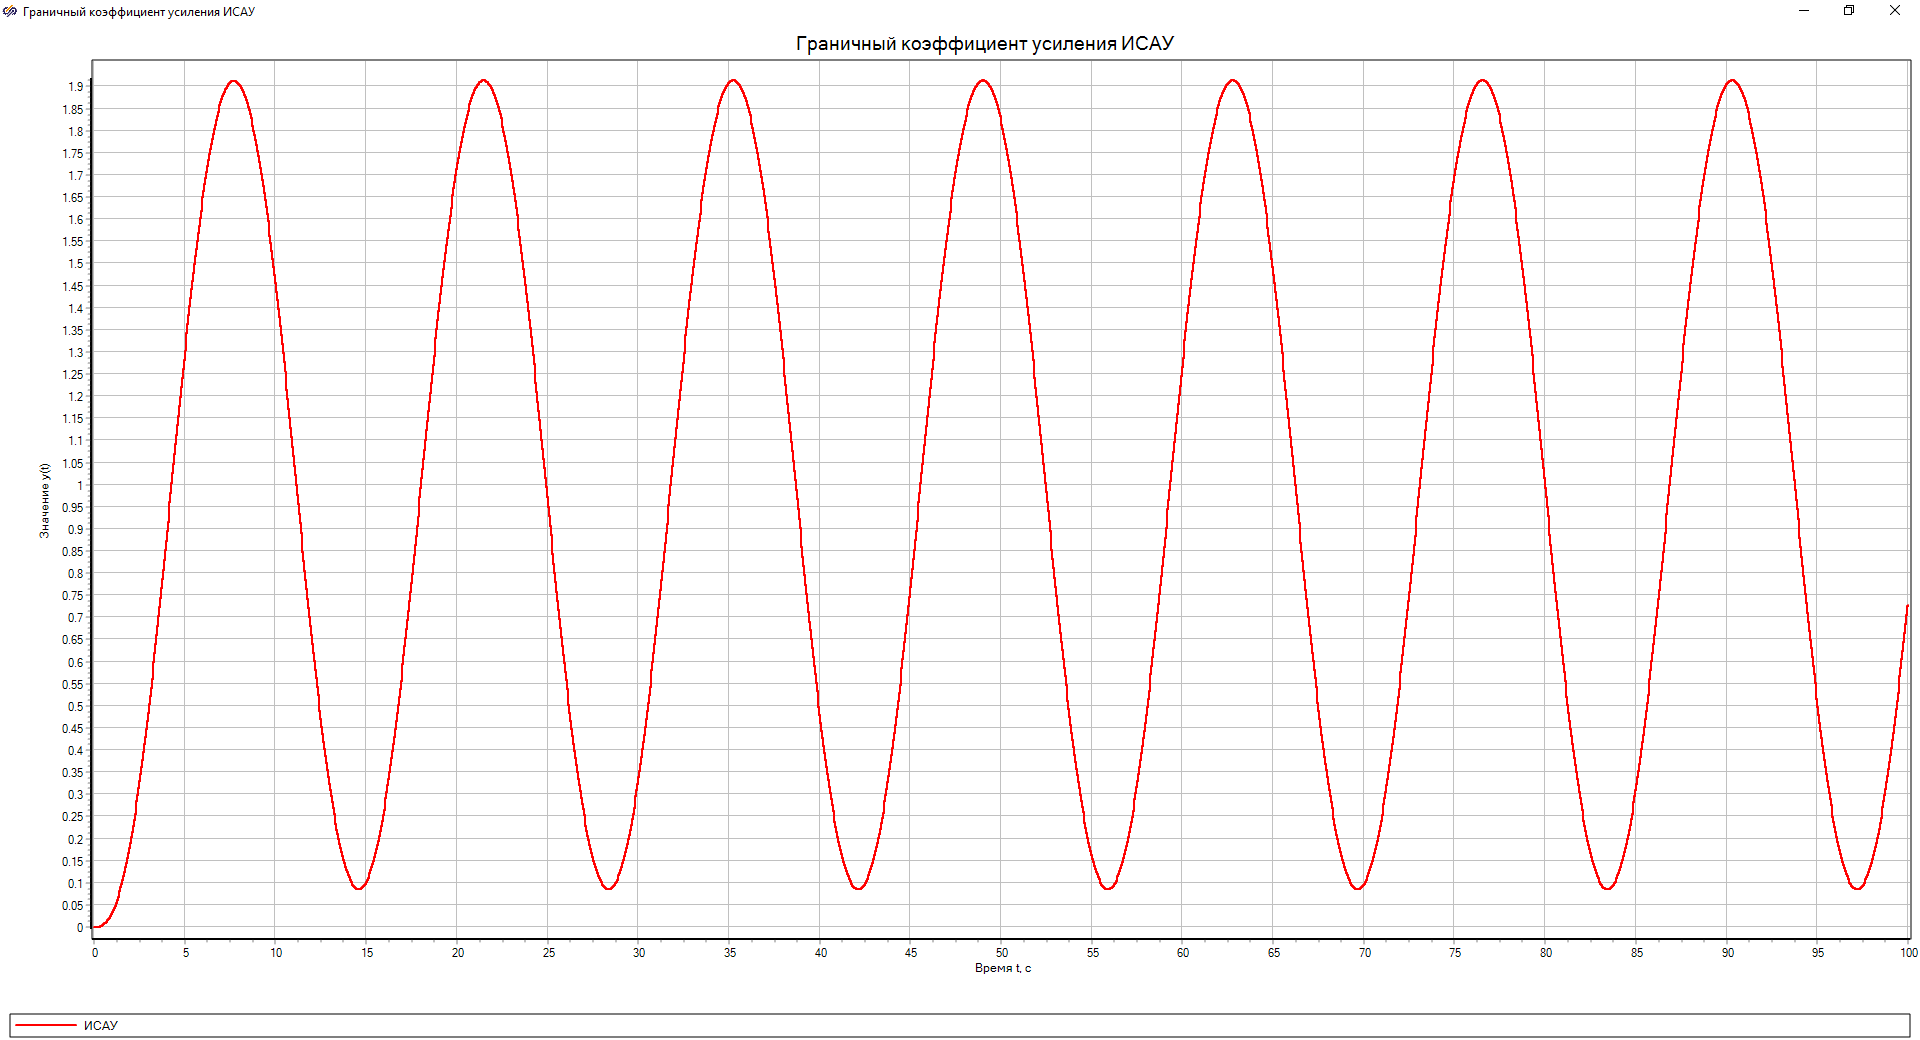
\includegraphics[width=.75\textwidth]{png/graph4.png}
		\caption{Незатухающий переходной процесс для системы с $T_1 = 2$ с и $T=0,01$ c}
		\label{graph4}
	\end{figure}
	
	В результате ряда экспериментов были получены данные, которые представлены в табл. \ref{table2}. Как видно из таблицы, по сравнению с непрерывной системой, предельное значение добротности уменьшилось максимально на 24\%, что значительно.
	
	\begin{table}[]
		\resizebox{\columnwidth}{!}{%
			\begin{tabular}{|c|cccccc|}
				\hline
				\multirow{2}{*}{$T_1$, с} & \multicolumn{6}{c|}{Предельная добротность $k_\text{пр}$}                                                                                                                                    \\ \cline{2-7} 
				& \multicolumn{1}{c|}{САУ}   & \multicolumn{1}{c|}{ИСАУ $T=0.01$} & \multicolumn{1}{c|}{ИСАУ $T=0.05$} & \multicolumn{1}{c|}{ИСАУ $T=0.1$} & \multicolumn{1}{c|}{ИСАУ $T=0.25$} & ИСАУ $T=0.5$ \\ \hline
				1                                           & \multicolumn{1}{c|}{0,665} & \multicolumn{1}{c|}{0,664}         & \multicolumn{1}{c|}{0,655}         & \multicolumn{1}{c|}{0,644}        & \multicolumn{1}{c|}{0,616}         & 0,573        \\ \hline
				2                                           & \multicolumn{1}{c|}{1,07}  & \multicolumn{1}{c|}{1,065}         & \multicolumn{1}{c|}{1,042}         & \multicolumn{1}{c|}{1,014}        & \multicolumn{1}{c|}{0,943}         & 0,845        \\ \hline
				3                                           & \multicolumn{1}{c|}{1,33}  & \multicolumn{1}{c|}{1,323}         & \multicolumn{1}{c|}{1,290}         & \multicolumn{1}{c|}{1,25}         & \multicolumn{1}{c|}{1,145}         & 1,008        \\ \hline
			\end{tabular}%
		}
		\caption{Предельные значения добротности для разных параметров ИСАУ}
		\label{table2}
	\end{table}
	
	Границы устойчивости для разных периодов квантования представлены на рис. \ref{gr_ust}. Здесь хорошо видно, что большие значения квантования уменьшают область устойчивости системы.
	
	\begin{center}
		\begin{tikzpicture}
			\begin{axis}[
				xlabel={$T_1$},
				ylabel={$k_\text{пр}$},
				xmin=0, xmax=3.25,
				xtick distance = 1,
				ytick distance = 0.25,
				xlabel style={above right},
				ylabel style = {above right},
				ymin=0.5, ymax=1.5,
				axis lines = center,
				width=.7\textwidth,
				clip=false
				]
				
				\addplot[
				]
				coordinates {
					(1,0.665)(2,1.07)(3,1.33)
				}
				node [pos=1, above left] {САУ};
	
				\addplot[
				]
				coordinates {
					(1,0.664)(2,1.065)(3,1.323)
				}
				node [pos=1, above right] {$T=0.01$};
				
				\addplot[
				]
				coordinates {
					(1,0.655)(2,1.042)(3,1.29)
				}
				node [pos=1, right] {$T=0.05$};
				
				\addplot[
				]
				coordinates {
					(1,0.644)(2,1.014)(3,1.25)
				}
				node [pos=1, below right] {$T=0.1$};
				
				\addplot[
				]
				coordinates {
					(1,0.616)(2,0.943)(3,1.145)
				}
				node [pos=1, right] {$T=0.25$};
				
				\addplot[
				]
				coordinates {
					(1,0.573)(2,0.845)(3,1.008)
				}
				node [pos=1, right] {$T=0.5$};
			\end{axis}
		\end{tikzpicture}	
		\captionof{figure}{Границы устойчивости для разных периодов квантования}
		\label{gr_ust}
	\end{center}
	
	\section{Выводы}
	
	Было исследовано влияние введения дискретизации по времени в непрерывных системах. Для малых периодов квантования отличие между ИСАУ и САУ практически не наблюдалось. С увеличением периода квантования динамические свойства и запас по устойчивости ухудшались. 
	
	Если сравнивать непрерывные и импульсные системы в установившемся режиме, то при условии, что устойчивость при введении дискретизации не нарушается -- установившийся режим в системах совпадает. А следовательно и совпадают показатели ошибки регулирования.
	
		
\end{document}
